\chapter{Grundlagen}

\section{Duckietown-Simulator}

\subsection{Übersicht}

Der \href{https://github.com/duckietown/gym-duckietown}{Duckietown-Simulator} ist ein in \href{https://www.python.org/}{\texttt{Python}} und \href{https://www.opengl.org/}{\texttt{OpenGL}} \acf{bzw} \href{http://pyglet.org/}{\texttt{Pyglet}} geschriebener Simulator für das \glqq Duckietown-Universum\grqq. Der Simulator bietet die Möglichkeit Duckiebots (Agenten) in einer beliebigen Duckietown-Umgebung zu platzieren und die Agenten darin zu navigieren. Eine Duckietown-Umgebung beinhaltet hierbei eine Menge von befahrbaren Straßenstücken, eine Menge Hindernisse, sowie nicht befahrbare Umgebungsabschnitte. \cite{gym_duckietown} \\

\begin{figure}[H]
	\centering
	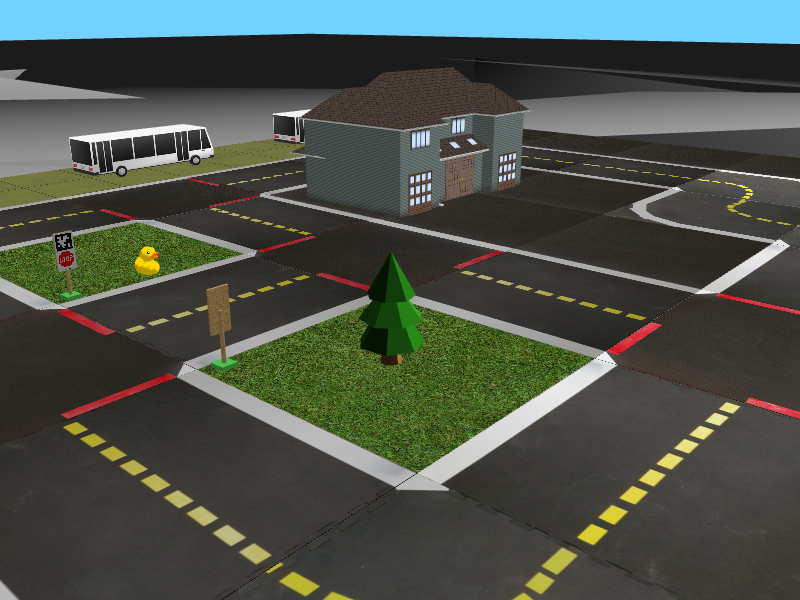
\includegraphics[width=0.8\textwidth]{kapitel2/images/duckietown-gym.png}
	\label{fig:duckietown-gym}
	\caption{Duckietown-Simulator}
\end{figure}

Der Simulator ist schnell, quelloffen und ausgesprochen anpassungsfähig. Er wurde zunächst für die einfache Linienverfolgung konzipiert und wurde dann im Laufe der Zeit zu einem voll funktionsfähigen Simulator für autonom fahrende Fahrzeuge, insbesondere im Bezug zur künstlichen Intelligenz. \cite{gym_duckietown}

\subsection{Duckietown-Umgebung}

In einer Duckietown-Umgebung wird die Umwelt für einen Duckie-Bot definiert. Ein Duckiebot kann diese Umgebung dann observieren und sich in dieser bewegen. Eine Duckietown-Umgebug wird dabei aus verschiedenen Kacheln und Objekten aufgebaut. Bei den Kacheln wird zwischen befahrbaren und nicht befahrbaren Kacheln unterschieden. 

\begin{figure}[H]
	\centering
	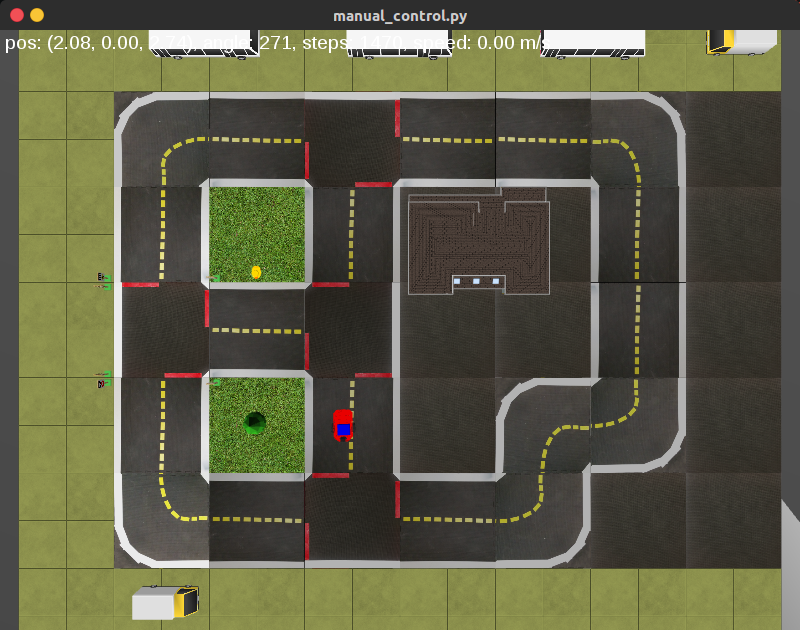
\includegraphics[width=0.8\textwidth]{kapitel2/images/duckietown-umgebung.png}
	\label{fig:duckietown-umgebung}
	\caption{Beispielhafte Duckietown-Umgebung}
\end{figure}


\subsection{Duckiebot}

Ein Duckiebot ist ein mobiler Roboter mit Differenzialantrieb, der seine Umgebung über eine Kamera wahrnehmen kann. Er kann mittels eines Steuerbefehls in der Umgebung navigiert werden. \cite{duckietown_platform}

\begin{figure}[H]
	\centering
	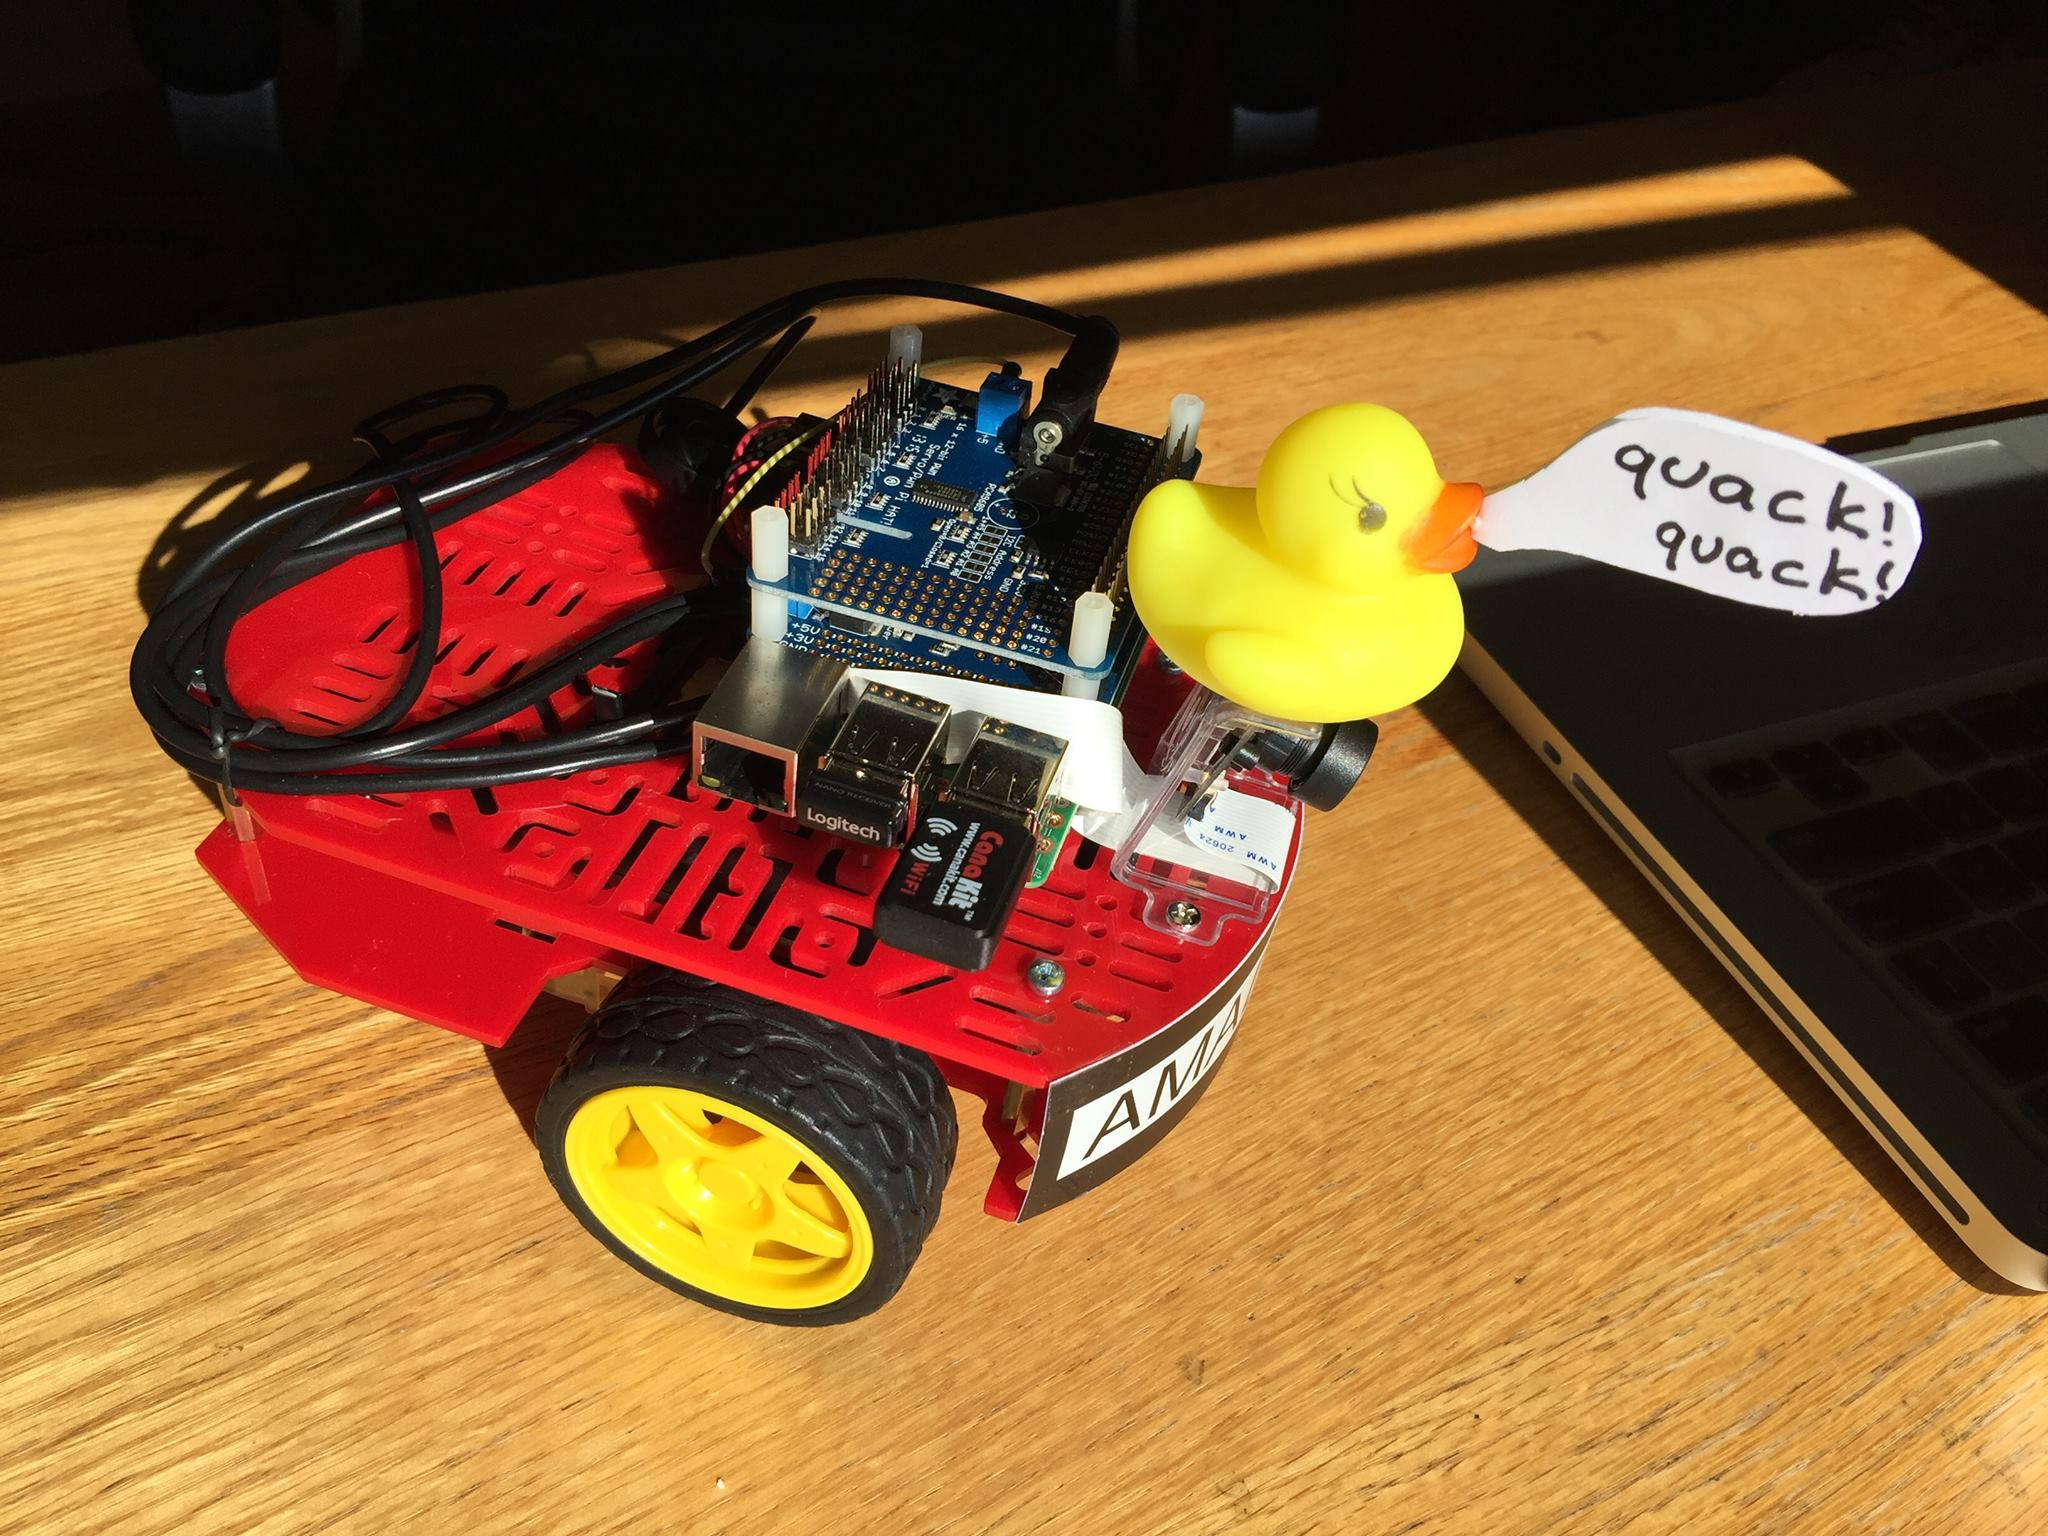
\includegraphics[width=0.6\textwidth]{kapitel2/images/duckiebot.jpg}
	\label{fig:duckiebot}
	\caption{Duckiebot}
\end{figure}

\section{Aufgabenstellung}

Das Ziel des Teamprojekts war es, die relative Position eines Duckiebots im Bezug zur rechten Fahrbahnmarkierung eines Straßenabschnittes zu ermitteln. Die relative Position beinhaltet hierbei den Abstand zur Seitenmarkierung, sowie die Orientierung zu dieser. Dabei soll maschinelles Lernen zum Einsatz kommen, um die Position des Duckiebots inferieren zu können, unabhängig von der eingesetzten Duckietown-Umgebung. 


